\documentclass[../../dissertation.tex]{subfiles}
\begin{document}

%TODO: Decidir se ficam 3 pontos verticais.
\begin{figure}[h]
        \[ \Qcircuit @C=1em @R=.7em {& \targ    & \qw      & \qw      & \qw      & \qw \\
        			  & 	     & 	        &          &          &  . \\
        			  & 	     & 	        &          &          &  . \\
        			  & 	     & 	        &          &          &  . \\
        			  & \ctrl{-4} & \targ   & \qw      & \qw      & \qw \\
        			  & \ctrl{-1} & \ctrl{-1} & \targ    & \qw      & \qw\\ 
        			  & \ctrl{-1} & \ctrl{-1} & \ctrl{-1} & \qw      & \qw
			  } \]
	\centering
	\caption{Douglas wang increment}
	\label{fig:coinedIncrement}
\end{figure}

\begin{figure}[h]
        \[ \Qcircuit @C=1em @R=.7em {& \targ    & \qw      & \qw      & \qw      & \qw \\
        			  & 	     & 	        &          &          &  . \\
        			  & 	     & 	        &          &          &  . \\
        			  & 	     & 	        &          &          &  . \\
        			  & \ctrlo{-4} & \targ   & \qw      & \qw      & \qw \\
        			  & \ctrlo{-1} & \ctrlo{-1} & \targ    & \qw      & \qw\\ 
        			  & \ctrlo{-1} & \ctrlo{-1} & \ctrlo{-1} & \qw      & \qw
			  } \]
	\centering
	\caption{Douglas wang Decrement}
	\label{fig:coinedDecrement}
\end{figure}

%TODO; Descobrir como separar a moeda do resto do circuito. Adicionar node e subnode?
\begin{figure}
	\[ \Qcircuit @C=1em @R=0em { &\qw & \multigate{4}{incr} &  \multigate{4}{decr} & \qw \\
				     &\qw & \ghost{incr} & \ghost{decr} & \qw \\
               			     &\qw & \ghost{incr} & \ghost{decr} & \qw \\
            			     &\qw & \ghost{incr} & \ghost{decr} & \qw \\
            			     &\qw & \ghost{incr} & \ghost{decr} & \qw \\ 
				     &    &              &              &     \\
				     &    &              &              &     \\
				     &    &              &              &     \\
				     &\gate{H} & \ctrl{-2} & \ctrlo{-2} & \qw 
		          } \]
	\centering
	\caption{Douglas wang coined quantum walk circuit}
	\label{fig:coinedDecrement}
\end{figure}

%TODO: Usar o artigo do douglas wang para saber o que escrever.
\begin{figure}[!h]
	\centering
	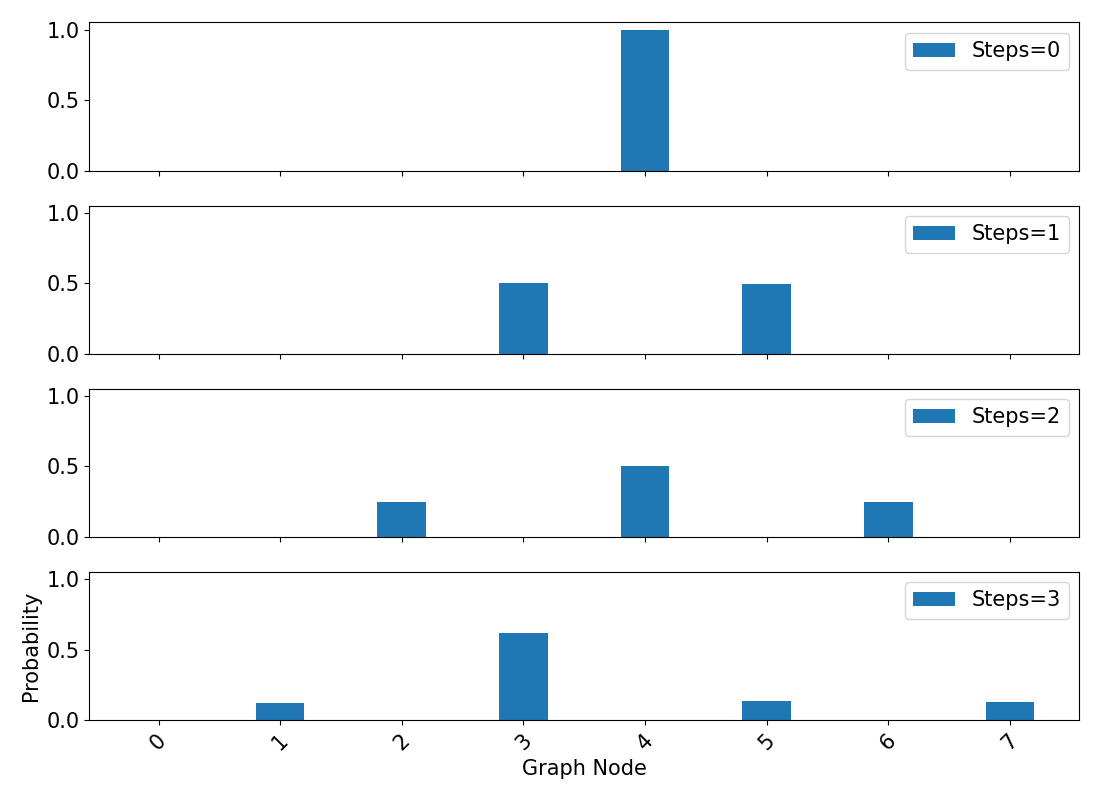
\includegraphics[scale=0.40]{img/Qiskit/CoinedQuantumWalk/CoinedQW_N3_S0123.png}
	\caption{Probability distribution for the staggered quantum walk on a line after 50 steps, with initial condition $\ket{\Psi(0)}=\frac{\ket{0}+\ket{1}}{\sqrt{2}}$, for multiple angles.} 
	\label{fig:fig5}
\end{figure}

\end{document}
